\documentclass[a4paper,10pt]{report}

% Graphics.
\usepackage{graphicx, subfigure}
\usepackage{caption}

% Language.
\usepackage[english]{babel}

% Math packages.
\usepackage{amssymb}
\usepackage{amstext}
\usepackage{amsmath}

% Wide pages.
%\usepackage[margin=0.5in]{geometry}

% Monospace font.
\usepackage[T1]{fontenc}
\usepackage{inconsolata}

% Url.
\usepackage{url}

\newcommand{\tab}{\hspace*{1em}}

\begin{document}

\title{Herding sheep \\
	\large Comparing Different Modalities for Game Interaction}
\author{Bas Bootsma (0719080) \and Bas Kooiker (0815381) \and Roland Meertens (3009653) \and Thomas Planting (3030938)}
\date{\today}
\maketitle
\tableofcontents

%%%%%%%%%%%%%%%%%%%%%%%%%%%%%%%%%%%%%%%%%%%%%%%%%%%%%%%%%%%%%%%%%%%%%%%%%%%%%%%
% Introduction
%%%%%%%%%%%%%%%%%%%%%%%%%%%%%%%%%%%%%%%%%%%%%%%%%%%%%%%%%%%%%%%%%%%%%%%%%%%%%%%
\chapter{Introduction}
\label{chap:introduction}

At the dawn of the digital information era, personal computers used to be controlled almost entirely via their keyboards with DOS systems. 
In the mid to late 1980's, the mouse made its entry into almost every personal computer system.
Today in the 21st century, many other input modalities have been incorporated into computer systems.
Often, these modalities are much more humanlike than a mouse and keyboard. 
Think of touch, voice recognition and motion sensors, these are actual ways for a computer to interpret information from the world, instead of hardcoded commands from the mouse and keyboard. 
In many ways, these modalities can be compared with actual human senses, which makes interacting with them more intuitive and natural \cite{earnshaw2001frontiers}.
In the 21st century, computers are starting to adapt to humans instead of the other way around.

With so many interaction modalities becoming available, determining which fits best for what situation is a real challenge.
To help research this, we have set up a comparative experiment between the user experience of a game when played on a touchtable compared to when played with a mouse on a personal computer.
For this research, we have implemented a simple puzzle game called "Herdinator". 
The goal of this game is to herd as many agents (sheep) as possible to a goal area in the middle of the screen.
The players have two tools at their disposal to influence the movements of the sheep, one to attract the sheep and one to repulse them.
A detailed specification of the game will be given in section~\ref{chap:specification}.
The game can be played both on a personal computer and on a multi-touch table we have set up for this project. A description of the multi-touch table is given in section~\ref{HardwareComponents}
When playing on a personal computer, the users will interact with the game with a mouse.
When playing on our touchtable the users will interact with the game through the touch modality.

While many more input modalities have been incorporated into computer systems, there has not been a lot of research comparing the enjoyabilitiy of playing games between these two platforms. 
One paper that did inspire us is \cite{Tychsen2007}.
The authors of that paper compare the enjoyability of role playing games on tabletops and on computers.
They also present some useful analyzing tools. 
Our research focusses on puzzle games, and compares personal computers to touchtables.
We think more of this kind of research is warranted in an age in which both the popularity of gaming and the use of different ways to interact with computers are growing rapidly.
Our research question is: Will users prefer to use the touch modality or the mouse? 
We think it is more intuitive to drag objects by literally touching the "screen" (the touch-table) than to select them with a mouse and then drag them.
However, since we will be comparing a multi-touch table we had to set up ourselves with an industrially produced personal computer, there will probably be a difference in quality between the two platforms. If the accuracy of the touchtable is low it will likely be more frustrating than the personal computer.

Our hypothesis is: The user experience with the multi-touch table will be more positive than with the personal computer, unless the accuracy of the multi-touch table is low. \\\\
We will start with specifying the game we implemented in section \ref{chap:specification}, both informally and with the  GOMS (Goals Operators Methods Selection) modelling technique. 
Then we will give an overview of our implementation in section \ref{chap:implementation}, with a focus on the explicit design decisions that led to it.
After that we will discuss the usability study we performed in section \ref{chap:usabilitystudy} and present the results in section \ref{chap:results}. 
We finish with a discussion section \ref{chap:discussion}, in which we discuss the results of the usability study and possible future research. 

%%%%%%%%%%%%%%%%%%%%%%%%%%%%%%%%%%%%%%%%%%%%%%%%%%%%%%%%%%%%%%%%%%%%%%%%%%%%%%%
% Specification
%%%%%%%%%%%%%%%%%%%%%%%%%%%%%%%%%%%%%%%%%%%%%%%%%%%%%%%%%%%%%%%%%%%%%%%%%%%%%%%
\chapter{Specification}
\label{chap:specification}

\section{Informal specification}
We have created a sheepherding puzzle game, which can be played alone and cooperative with up to 4 players.
The game can be played both on a personal computer using a mouse or on a multi-touch table.
The game environment consists of a grass field with a herd of sheep and several special objects and actors in it.
The players have the task to herd the sheep to a specified goal area as fast as possible.
To do so, they have to select certain special objects and drag them to desired locations.

When the game is played on a personal computer, the objects can be dragged with the mouse. 
When the game is played on a touchtable, the objects can be dragged over the touchtable by dragging over it.
These objects will attract special actors, which in turn will attract or repulse the sheep.
The objects can be moved at any time, but there are only two objects in the game at a time.

The following special actors are in the game: \\

\begin{itemize}

\item
	Love sheep ("Maggie"): This will attract sheep.
\item
	Dog ("Balthazar"): This will drive the sheep away \\
\end{itemize}
The following special (moveable) objects are in the game:\\
\begin{itemize}
\item
	Whistle: This will attract the love sheep "Maggie".
\item
Cookie: This will attract the dog "Balthazar".\\
\end{itemize}

This amounts to one tool for attracting sheep and one for repulsing them. 
A sheep will only be attracted by the love sheep if it is within a certain specified range.
Likewise, a sheep will only be repulsed by the dog if it is within a specified range.
By default, sheep walk around semi-randomly, with a higher probability to walk to each other if 
If a sheep is attracted by the love sheep, it will have a higher probability of walking towards the love sheep each action.
If a sheep is repulsed by the dog, it will have a higher probability to walk away from the dog each action.
If a sheep is near both the love sheep and the dog, the repulsion from the dog will supersede the attraction by the love sheep.
If a sheep has reached the goal area, it is no longer affected by the dog and the love sheep, and will not be able to leave the goal area.
There is a "fence" around the goal area which blocks movement with two openings, one at the bottom and one at the top of the goal area.
The sheep and the agents can only pass through those openings. 
The player or players will get a score depending on the number of sheep that were collected when the timer ends.
If all the sheep are collected, bonus points will be assigned based on the time left.
When played with multiple players, they will all get equal score, thus making the game fully cooperative.

\section{GOMS specification}

\subsection{Touchtable}
Goal: Drive as many sheep as possible in the goal area.
\\
\tab Repeat until time runs out \\
\tab \tab Select \\
\tab  \tab \tab Goal: Attract sheep to position\\
\tab \tab \tab \tab choose location \\
\tab \tab \tab \tab Goal: attract lovesheep \\
\tab \tab \tab \tab \tab touch position of cookie \\
\tab \tab \tab \tab \tab drag cookie to desired location \\
\tab \tab \tab Goal: Drive sheep away from position\\
\tab \tab \tab \tab choose location \\
\tab \tab \tab \tab Goal: attract dog \\
\tab \tab \tab \tab \tab touch position of whistle \\
\tab \tab \tab \tab \tab drag whistle to desired location\\

\subsection{Personal Computer}
Goal: Drive as many sheep as possible in the goal area.
\\
\tab Repeat until time runs out \\
\tab \tab Select \\
\tab  \tab \tab Goal: Attract sheep to position \\
\tab \tab \tab \tab choose location \\
\tab \tab \tab \tab Goal: attract lovesheep \\
\tab \tab \tab \tab \tab click cookie \\
\tab \tab \tab \tab \tab drag cookie to desired location with mouse\\
\tab \tab \tab Goal: Drive sheep away from position\\
\tab \tab \tab \tab choose location \\
\tab \tab \tab \tab Goal: attract dog \\
\tab \tab \tab \tab \tab click whistle \\
\tab \tab \tab \tab \tab drag whistle to desired location with mouse\\

%%%%%%%%%%%%%%%%%%%%%%%%%%%%%%%%%%%%%%%%%%%%%%%%%%%%%%%%%%%%%%%%%%%%%%%%%%%%%%%
% Implementation
%%%%%%%%%%%%%%%%%%%%%%%%%%%%%%%%%%%%%%%%%%%%%%%%%%%%%%%%%%%%%%%%%%%%%%%%%%%%%%%
\chapter{Implementation}
\label{chap:implementation}

	%%% System Architecture %%%%%%%%%%%%%%%%%%%%%%%%%%%%%%%%%%%%%%%%%%%%%%%%%%%%%%%
	\section{System Architecture}
	\label{sec:system-architecture}
	In the following section we will give an overview of the architecture of the system and the individual components.
	The components are divided into three categories, namely hardware components, software components and the interaction between hardware and software components.

	%%%%% Hardware Components %%%%%%%%%%%%%%%%%%%%%%%%%%%%%%%%%%%%%%%%%%%%%%%%%%%
	\subsection{Hardware Components}
	\label{HardwareComponents}

		\subsubsection{Tabletop}
		The tabletop consists of a table where we replaced the table top with a glass plate with a layer of tracing paper on top.
		Underneath the glass plate a huge mirror is placed that reflects the projects image by the beamer. 
		Besides the mirror there is a small webcam that records everything that happens on the screen and everything that is visible through the tracing paper. 

		\begin{figure}[h!]
		\caption{The tabletop}
		\centering
		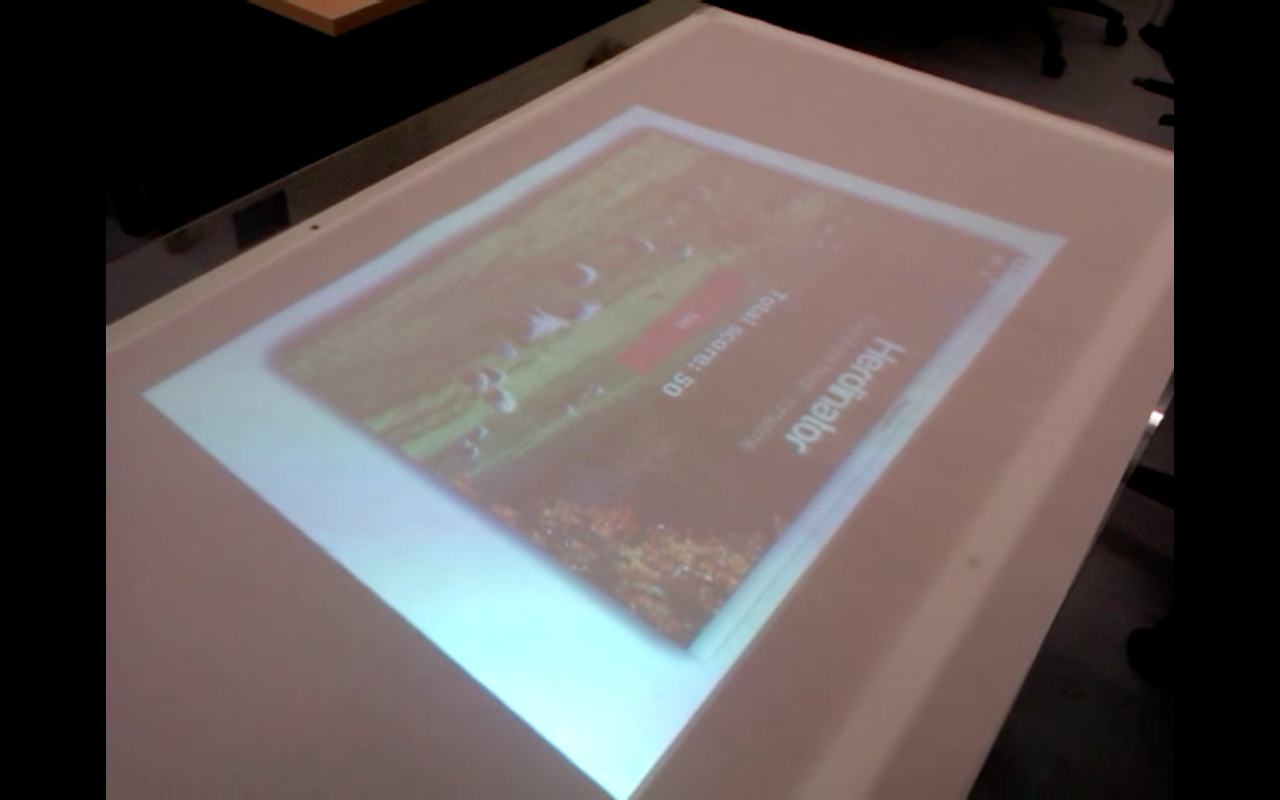
\includegraphics[width=0.5\textwidth]{images/tabletop}
		\end{figure}

		\subsubsection{Beamer}
		The beamer that projects an image on the tabletop is borrowed from our department and is a small portable beamer.
		The image that is projected is sharp enough for the user to get an accurate idea of what is happening on the screen. 
		As the projected image is not projected very wide the mirror in the tabletop is used. 

		\begin{figure}[h!]
		\caption{The tabletop}
		\centering
		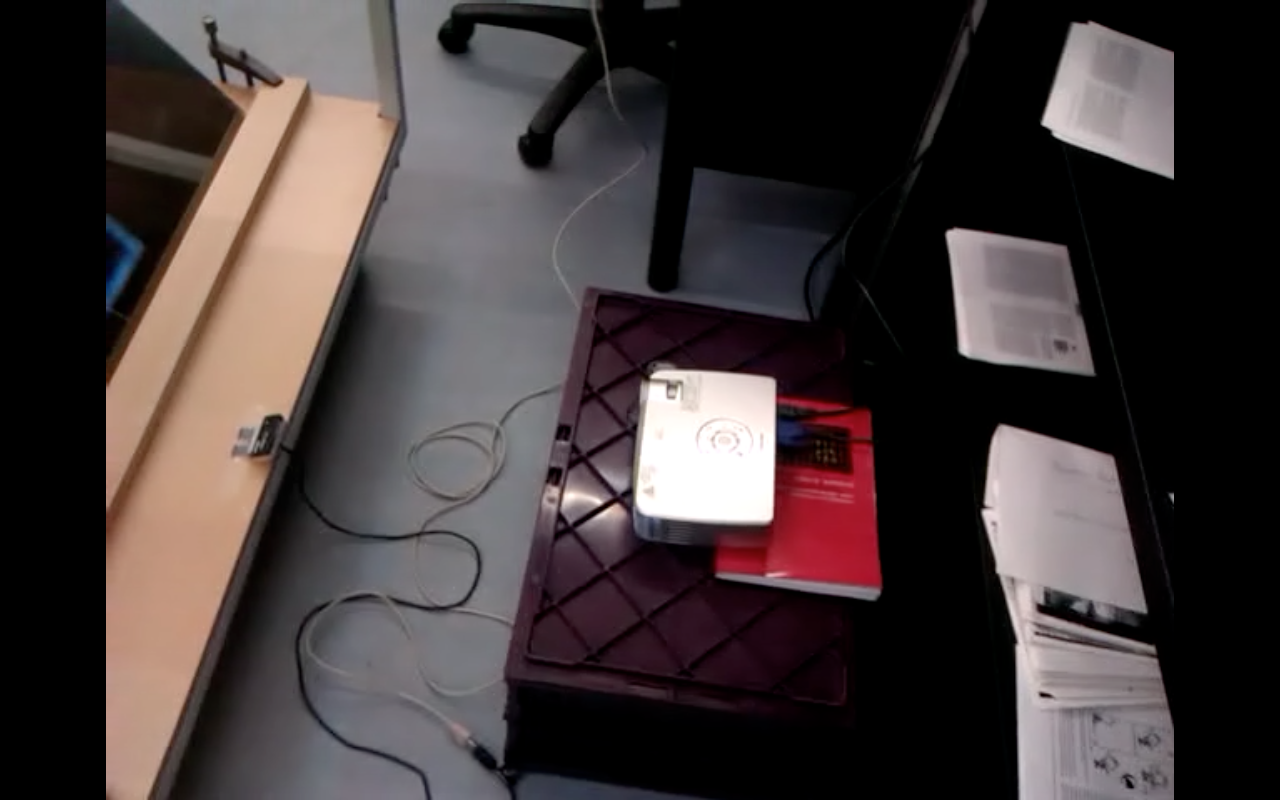
\includegraphics[width=0.5\textwidth]{images/beamer}
		\end{figure}

		\subsubsection{Webcam}
		The webcam used for our project is a simple consumer Microsoft Livecam. 
		Our webcam records in a medium quality high enough for our simple application. 
		Of course, using a better webcam would have improved our application but our current results were already acceptable. 

		\begin{figure}[h!]
		\caption{The webcam}
		\centering
		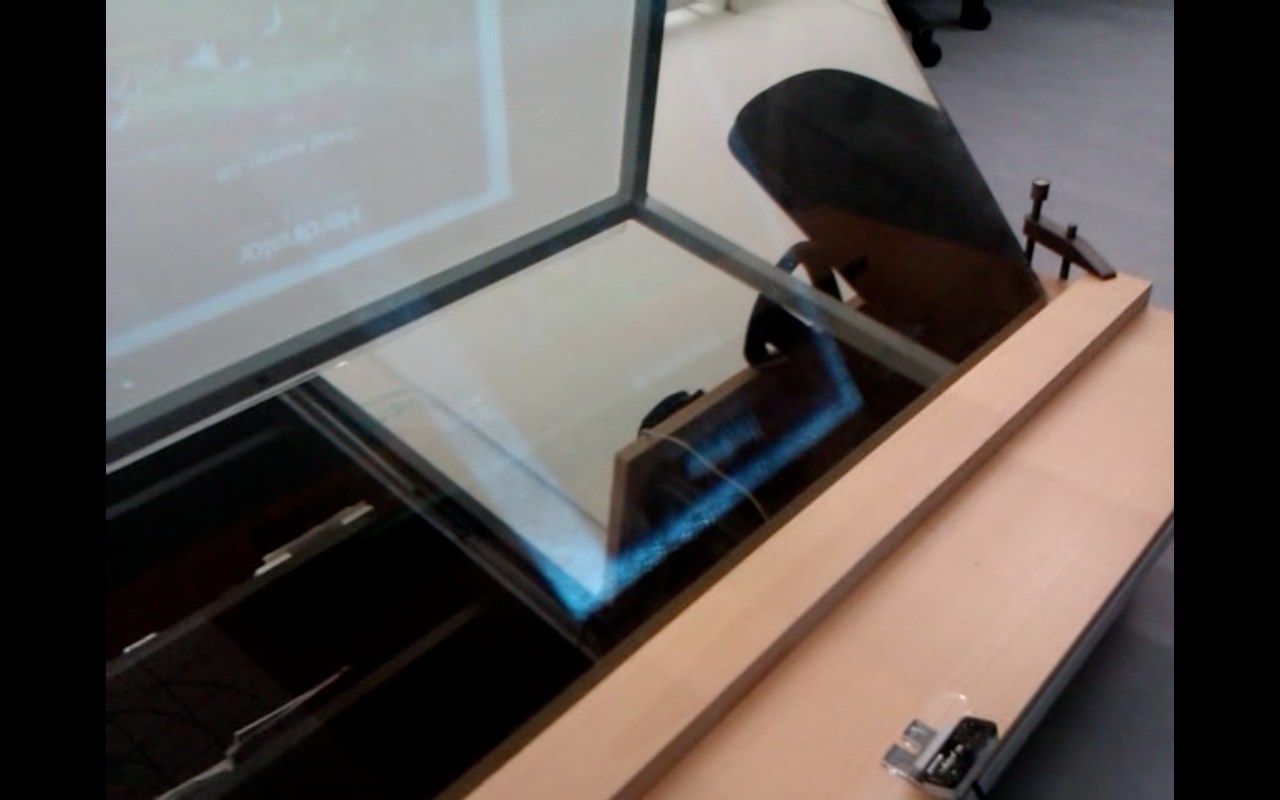
\includegraphics[width=0.5\textwidth]{images/webcam}
		\end{figure}

	%%%%%% Software Components %%%%%%%%%%%%%%%%%%%%%%%%%%%%%%%%%%%%%%%%%%%%%%%%%%
	\subsection{Software Components}
	\label{sec:software-components}
	In the following section an overview is given of the individual software components, namely the \emph{game}, the \emph{server} and the \emph{Android application}.
	An overview of the communication protocol between the server and the Android application is described i section~\ref{sec:communication-protocol}.

		%%%%%%% Game %%%%%%%%%%%%%%%%%%%%%%%%%%%%%%%%%%%%%%%%%%%%%%%%%%%%%%%%%%%%%%%%
		\subsubsection{Game}
		The game itself is written in Java and is built using the open source game platform Slick2D \cite{Slick2D}.
		Slick2D is primarily a wrapper around LWJGL \cite{LWJGL} and provides certain functionality to make it easier to develop games.
		LWJGL is primarily intended to allow developers easy access to certain libraries, like OpenGL, OpenCL, OpenAL, etc., to be used effectively and efficiently in Java.
		On itself LWJGL is not very suited to develop games with, however Slick2D adds extra functionality on top of LWJGL, like a game loop, a state switching mechanism, animations, etc.
		
		The game itself is divided into several parts, each containing many different objects of which most are not very important nor interesting to discuss.
		Therefor we will only discuss the core parts, which are the different states, the \emph{GameManager}-object and the \emph{Map}-object to get reasonable overview of the game.
		
		\paragraph{States}
		A small, but useful, feature of Slick2D is that it contains a state switching mechanism.
		This allowed us to create several states from which you can switch to any state.
		In figure~\ref{fig:game-state-diagram} an overview is given of the different states and in what way one can switch to another state through the normal usage of the game.
		The game starts in the \emph{LoadingState} after which it automatically transition to the \emph{ModalitySelectorMenuState}.
		In this state the user is able to select, via buttons on the screen, which modality it wants to use to play the game with.
		If the mouse/touch modality is chosen the game will transition to the \emph{ModalityMouseAndTouchMenuState}.
		If the tangible modality is chosen the game will transition to the \emph{ModalityTangiblesMenuState}.
		In both states the user is either able to go back or start the game after the appropriate preparations have been made.
		In the \emph{GameState} the actual game is run.
		If one of the two ending conditions, namely herding all the sheep or no more time left, has been reached the game will transition to the \emph{GameScoreMenuState}.
		In this state the user is presented with the score and given the only possibility to exit the game.
		There used to be the possibility of going back to the \emph{ModalitySelectorMenuState}, however there were some issues in resetting the game properly, thus we have removed this feature.
		
		\begin{figure}
			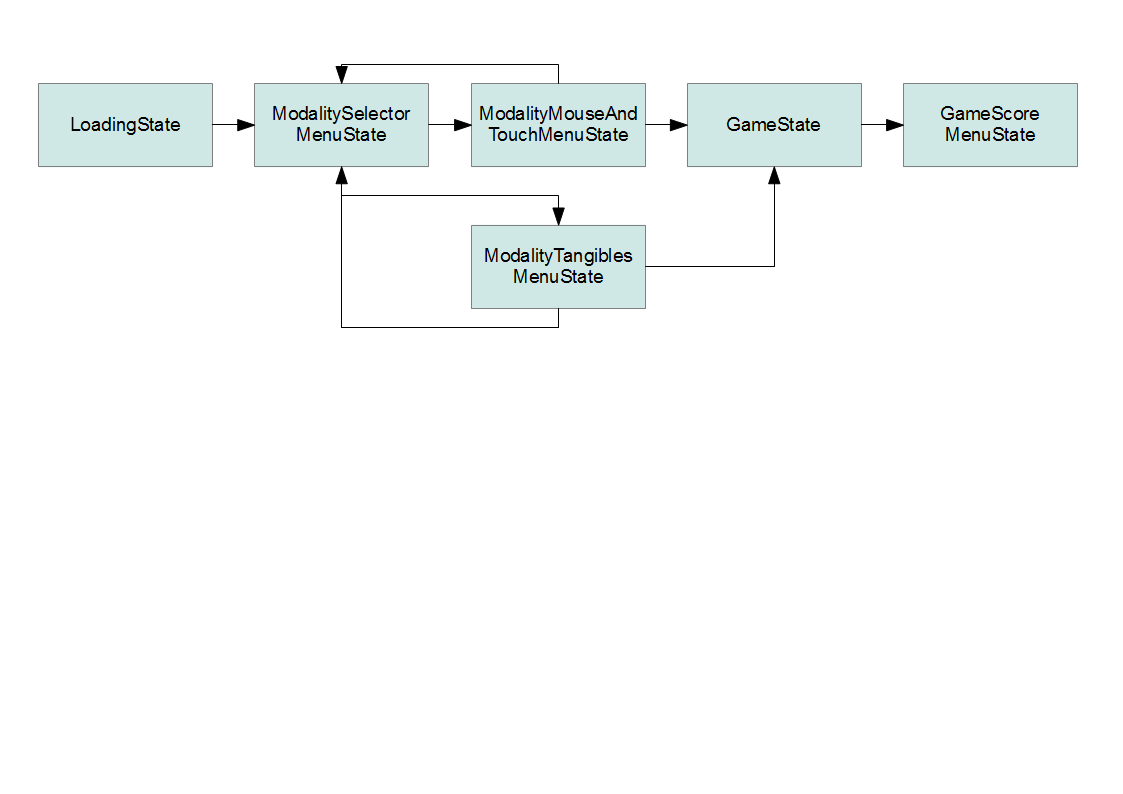
\includegraphics[width=\columnwidth]{images/game-state-diagram.png}
			\caption{Overview of the different states in the game.}
			\label{fig:game-state-diagram}
		\end{figure}
		
		\paragraph{GameManager}
		With the state switching mechanism of Slick2D it is not possible to transfer information between different states.
		Furthermore it is very practical to have a global object which can hold global information such that it is not necessary for each class to hold 
		Therefor we have created the \emph{GameManager}-object.
		\emph{GameManager} is a global singleton-object, meaning only a single instance of the object is available.
		Each object of the game can read and write specific information from and to the \emph{GameManager}.
		For example, \emph{GameManager} holds information about the current map being played and which players are currently playing the game.		
		
		\paragraph{Map}
		Arguably the most important object of the game is the \emph{Map}-object.
		\emph{Map} is primarily a container-object, holding many other objects, like sheep, dogs, cookies, etc.
		Furthermore it also contains functionality with which it is possible to perform correct moving and pathfinding behavior.
		Since \emph{Map} is one of the objects many other objects need to be aware of, it is also available through \emph{GameManager}.

	%%%%% Server %%%%%%%%%%%%%%%%%%%%%%%%%%%%%%%%%%%%%%%%%%%%%%%%%%%%%%%%%%%%%%%%
	\subsubsection{Server}
	The server has a key role in our setup.
	It handles the communication between the Android application and the game.
	For the server a portable version of Tomcat was used which is started at runtime every time the game starts.
	On the server we ran a single servlet which would handle all the communication between the server and the Android application.
	This setup is very flexible, since no one needs to have Tomcat installed and configured on their system.
	Furthermore it allows for a tight coupling between the game and the server application.
	On the one hand a tight coupling can be seen as a disadvantage since it becomes difficult to separate the server from the game.
	On the other hand it also saves a lot of time trying to built a suitable interface between the server and the game.
			
	Since the server is tightly couple with the game it is able to access all the components of the game through \emph{GameManager}.
	Using \emph{GameManager} the server is able to add and remove players which connect respectively disconnect themselves.
	Furthermore the server is able to manipulate the selected objects from each player.
	With this setup it is possible for the game to become instantly aware of changes of the players or of the objects of the players.
	
	%%%%% Android Application %%%%%%%%%%%%%%%%%%%%%%%%%%%%%%%%%%%%%%%%%%%%%%%%%%%
	\subsubsection{Android Application}
	In our experiment the Android application with a smartphone is used as a tangible object.
	The Android application is used to communicate with the game via commands send to the server.
	The Android application consists of three screens, namely a \emph{login}-screen~\ref{fig:android-application-screen1}, a \emph{select object}-screen~\ref{fig:android-application-screen2} and a \emph{use selected object}-screen~\ref{fig:android-application-screen3}.
	In the \emph{login}-screen the user has to fill in the details of the server and the mark id which is on the back of the smartphone
	If the Android application is able to successfully connect to the server it switches to the \emph{select object}-screen.
	In the \emph{select object}-screen the user is able to select which object it wants to use.
	In our case there are only two objects to choose from, namely a whistle and a cookie.
	Once the user has selected an object the Android application switches to the \emph{use selected object}-screen.
	In the \emph{use selected object}-screen the user is able to use the object, by pressing it.
	If the object is used and the smartphone is placed on the interactive table it will be registered by the game and actors can act accordingly.
	If the user wants to select a different object it can perform a horizontal backwards swipe to return to the \emph{select object}-screen.
	
	\begin{figure}[ht]
		\begin{minipage}[b]{0.30\linewidth}
			\centering
			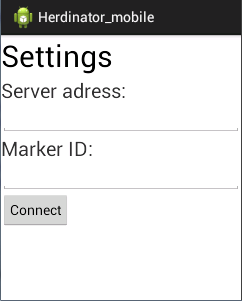
\includegraphics[width=\textwidth]{images/android-application-screen1.png}
			\caption{\emph{Login}-screen}
			\label{fig:android-application-screen1}
		\end{minipage}
		\hspace{0.1cm}
		\begin{minipage}[b]{0.30\linewidth}
			\centering
			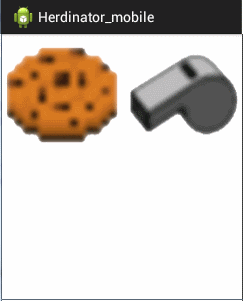
\includegraphics[width=\textwidth]{images/android-application-screen2.png}
			\caption{\emph{Select object}-screen}
			\label{fig:android-application-screen2}
		\end{minipage}
		\hspace{0.1cm}
		\begin{minipage}[b]{0.30\linewidth}
			\centering
			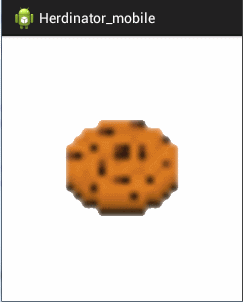
\includegraphics[width=\textwidth]{images/android-application-screen3.png}
			\caption{\emph{Use selected object}-screen}
			\label{fig:android-application-screen3}
		\end{minipage}
	\end{figure}

	%%%%% Interaction Between Hardware and Software Components %%%%%%%%%%%%%%%%%%
	\subsection{Interaction Between Hardware and Software Components}
	@TODO: Introduction...

	\subsubsection{reacTIVision}
	\label{sec:reactivision}
	reactTIVision is a software component that is able to detect both finger touches on a screen and specific markers. 
	The source image (taken from the webcam under the table) is first converted to a black and white image with an adaptive thresholding algorithm. 
	This image is converte	d into black and white regions, which is searched for unique sequences encoded into the fiducial symbols. \cite{reactivision}.
	At every frame it detects what markers are present and sends the corresponding event as described in section \ref{sec:tuioprotocol}

	\subsubsection{Community Core Vision}
	\label{sec:communitycorevision}	
	Community Core Vision (CCV) is a computer vision program that takes our video input stream (taken from the webcam under the table) and outputs tracking data. \cite{ccv}.
			Several features of CCV include several filters, input and output switchers and a calibration mode. 
	Using image processing CCV checks for the blobs that represent the tops of the fingers of the user. 
	The locations and ID's of these blobs are send using the TUIO protocol described in section \ref{sec:tuioprotocol}.
	\begin{figure}[h!]
		\caption{The game}
		\centering
		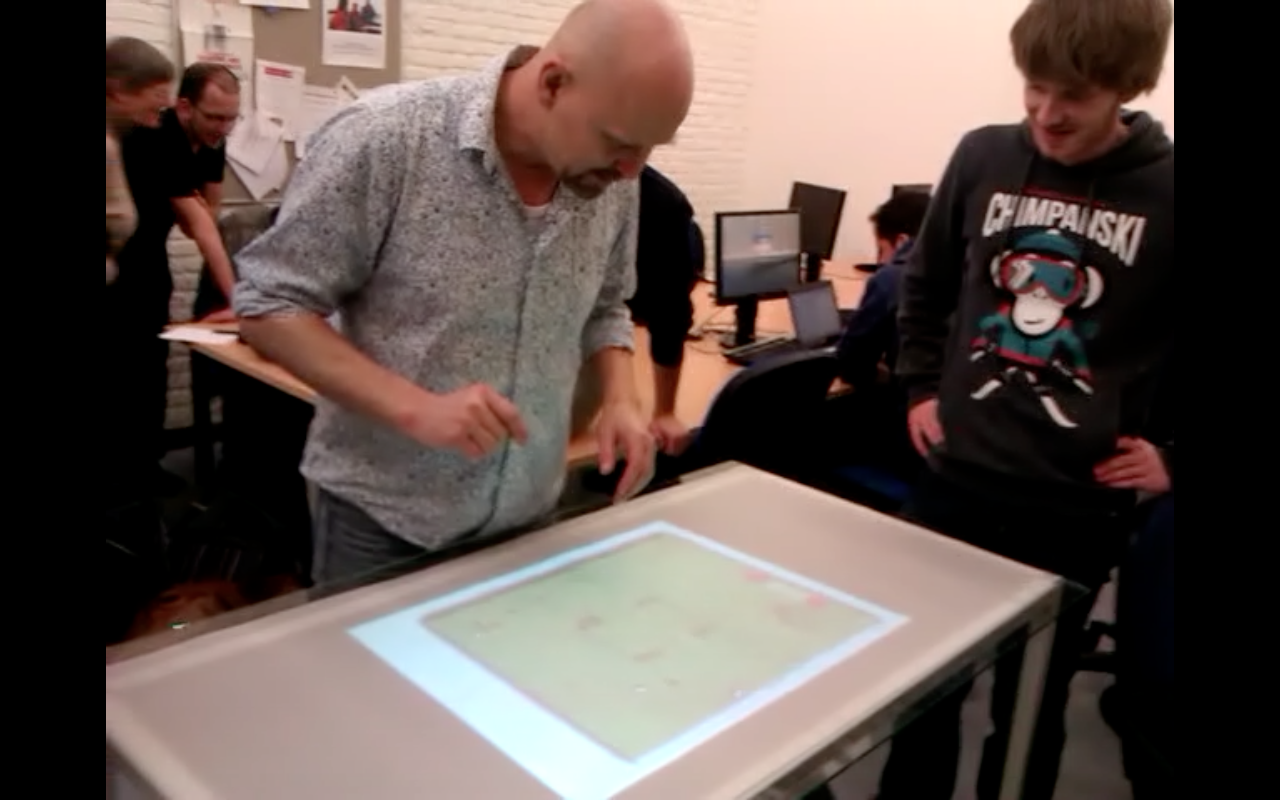
\includegraphics[width=0.5\textwidth]{images/tafelgebruik}
	\end{figure}
	
	\subsubsection{TUIO Protocol}
	\label{sec:tuioprotocol}
	The TUIO Protocol consists of a series of event-based communication using OSC messages over port 3333. \cite{tuioProtocol}. 
	Using a JAVA library our program catches these messages and calls an event every time a:
	\begin{enumerate}
		\item Finger is added to the screen;
		\item Finger is removed from the screen;
		\item Finger moved on the screen;
		\item Marker is added to the screen;
		\item Marker is removed from the screen;
		\item Marker is moved on the screen.
	\end{enumerate}
	
	These events also include a TUIOPoint object that contains among other the:
	\begin{enumerate}
		\item Location of the finger or marker;
		\item ID of the finger or marker.
	\end{enumerate}
	Using these events the objects in our game are updated to their locations respective to the game on the screen. % Volgens mij nergens: as described in section \ref{@TODO: waar wordts dit uitgelegd?}.
			
%%% Communication Protocol %%%%%%%%%%%%%%%%%%%%%%%%%%%%%%%%%%%%%%%%%%%%%%%%%%%%		
\section{Communication Protocol}
\label{sec:communication-protocol}
In order for the server and the Android application to exchange information with each other we had to design a communication protocol.
The communication protocol is used by the Android application to execute certain commands to let the game "know" a certain action has to be performed.

The Android application exchange information through a request-response paradigm.
The Android application sends a specific HTTP request which is interpreted by the server after which the server responds with JSON-formatted messages.
In order to read and write the messages the JSON.simple~\cite{JSONsimple} library is used.
Since both the Android application and the server use the same JSON library to read and write the messages there would be no problems in exchanging them.
Using JSON-formatted messages has several advantages:
\begin{itemize}
	\item
		\textbf{Easy to read and write programmatically}:
		Even though in our case a library handles most of the work, other formats, like XML, require more effort to get working.
	\item
		\textbf{Easy to read}:
		JSON-formatted messages are clear and concise making it easy to understand en verify the messages by hand, which helps in debugging.
	\item
		\textbf{Easy to expand}:
		The current setup makes it easy to add extra information to the messages, for example an error message when the request is unsuccessful.
\end{itemize}

For each request-response the Android application initiates the communication by sending one of the predefined requests as can be found below.
The server handles the request and responds either successfully, of which the specification can be found below, or unsuccessfully.
The message for an unsuccessful response is simply: \texttt{\{success:false\}}.

	%%%%% Commands %%%%%%%%%%%%%%%%%%%%%%%%%%%%%%%%%%%%%%%%%%%%%%%%%%%%%%%%%%%%%%%%	
	\subsection{Commands}
	Below a list of all the accepted requests is given.
	In general a certain order is required in executing the request.
	For example, first one has to execute the \emph{connect}-command before one can execute the \emph{select}-command and only after a successful \emph{select}-command one can execute the \emph{use}-command.
	No specific overview of the possible orders in which they can be executed is given, since it should follow from the specification.
		
		\subsubsection{Connect}
		Request: \texttt{?action=connect\&markId=[INTEGER]} \\
		Returns: \texttt{\{success:true, phoneId:[INTEGER]\}} \\

		\noindent Using the \emph{connect}-command the Android application is able to connect itself with the server.
		The parameter \texttt{markId} is required and should contain the id which corresponds with the mark on the back of the phone.
		If the request is successful a unique identifier \texttt{phoneId} is returned which should be used for every other request made.

		\subsubsection{Disconnect}
		Request: \texttt{?action=disconnect\&phoneId=[INTEGER]} \\
		Returns: \texttt{\{success:true\}} \\

		\noindent Using the \emph{disconnect}-command the Android application is able to disconnect itself with the server.
		The parameter \texttt{phoneId} is required and denotes the unique identifier which is returned on a successful connect.
		After a successful request any subsequent request with the given \texttt{phoneId} will fail.

		\subsubsection{Select}
		Request: \texttt{?action=select\&phoneId=[INTEGER]\&item=[STRING]} \\
		Returns: \texttt{\{success:true\}} \\

		\noindent Using the \emph{select}-command the Android application is able to select an item.
		The parameter \texttt{phoneId} is required and denotes the unique identifier which is returned on a successful connect.
		The parameter \texttt{item} is required and denotes the item to be selected. The supported items are: \emph{whistle} and \emph{cookie}.

		\subsubsection{Use}
		Request: \texttt{?action=use\&phoneId=[INTEGER]} \\
		Returns: \texttt{\{success:true\}} \\

		\noindent Using the \emph{use}-command the Android application is able to use the selected item.
		The parameter \texttt{phoneId} is required and denotes the unique identifier which is returned on a successful connect.
		If an item is successfully selected using the \emph{select}-command the item will appear in the game, which makes it possible for actors to respond accordingly.

%%%%%%%%%%%%%%%%%%%%%%%%%%%%%%%%%%%%%%%%%%%%%%%%%%%%%%%%%%%%%%%%%%%%%%%%%%%%%%%
% Usability Study
%%%%%%%%%%%%%%%%%%%%%%%%%%%%%%%%%%%%%%%%%%%%%%%%%%%%%%%%%%%%%%%%%%%%%%%%%%%%%%%
\chapter{Usability Study}
\label{chap:usabilitystudy}

\section{Goals}
In this study we will investigate the effect of using user interfaces of different modalities on the user experience.
This effect will be evaluated on multiple measures: 
\begin{enumerate}
	\item The subjective user experience;
	\item Objective user performance.
\end{enumerate}

In order to evaluate the user experience, we use an own implementation of the AttrakDiff user interface evaluation framework.
AttrakDiff divides user experience in four different aspects: 
\begin{description}
  \item
		\textbf{Attractiveness}
		The perceptual quality of a user interface.
  \item
		\textbf{Hedonic quality - Identity}
		To what extend users can identify with a user interface.
  \item
		\textbf{Hedonic quality - Stimulation}
		To what extend the user interface motivates users.
  \item
		\textbf{Pragmatic quality}
		The usability of a user interface.
\end{description} 

For different kinds of applications, different aspects from this framework will have a higher priority in the design process.
In most professional software, pragmatic quality will have the highest priority as reliability and performance quality are most important.
Also the hedonic identity quality is important as users should feel comfortable using it.
In professional design software, as another example, stimulation is a very important aspect.
In these interfaces, where users are in a creative process, users should always be stimulated as much as possible.
In games, interfaces which are mainly used for entertainment, the pragmatic quality is of lesser importance if the attractiveness and stimulating quality of the interface is high enough.
 
The objective performance of the users on different interaction modalities is measured by the game score that is implemented in the game.
This score is dependent on both the speed and the accuracy of the user.

%%%%%%%%%%%%%%%%%%%%%%%%%%%%%%%%%%%%%%%%%%%%%%%%%%%%%%%%%%%%%%%%%%%%%%%%%%%%%%%
% Results
%%%%%%%%%%%%%%%%%%%%%%%%%%%%%%%%%%%%%%%%%%%%%%%%%%%%%%%%%%%%%%%%%%%%%%%%%%%%%%%
\chapter{Results}
\label{chap:results}

A total of ten subjects participated in the experiment. We counter-balanced by having half of the participants start the experiment with the touch modality condition and the other half with the mouse modality. Each of the participants played the game using either of the modalities, filled in a questionnaire, played the game with the other modality, and filled in the same questionnaire again. Figure \ref{fig:pairs} shows the results for the rating of the word pairs comparing the two modalities. Figure \ref{fig:scores} shows the same results averaged over the four categories of word pairs. 

These results show that on average, the mouse modality interaction is rated higher on all categories except on hedonic stimulation quality. As mentioned before, in games or other entertainment purposes, this quality is of higher importance than the other qualities. The pairwise ratings show that all the words concerning stimulating quality are rated higher for the touch modality that the mouse modality. Another notable difference is that even though on average the touch modality is rated lower on the hedonic identity aspect, it is rated higher for the word 'brings me closer to people'. Subject had noted that even though the touch table did not work perfectly in terms of finger tracking and detection, it did give the game a more 'open' feeling as it inclined other people to watch along, whereas the mouse modality had a more isolating effect on the user. 

Figure \ref{fig:cat_int} shows the average performance scores of the subjects for the two interaction modalities. The average score for the touch modality was significantly lower than the average score of the mouse modality. We suspect that this difference is mainly due to the bad functioning of the touch table. Users had much problems dragging and selecting the objects and lost much of their time with this during the game wheras this was not a problem at all with the mouse interaction.  

\begin{figure}
  \centering
  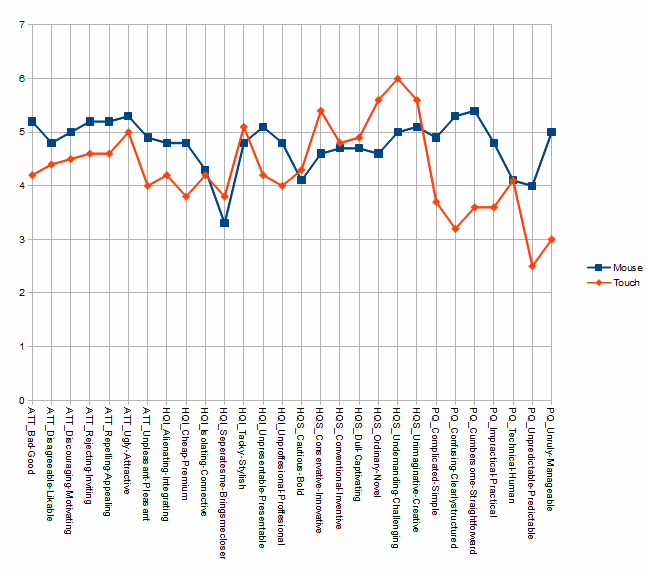
\includegraphics[width=0.8\textwidth]{images/pairs}
  \caption{The average rating per word pair for the two interface modalities.}
  \label{fig:pairs}
\end{figure}

\begin{figure}
  \subfigure[]{
    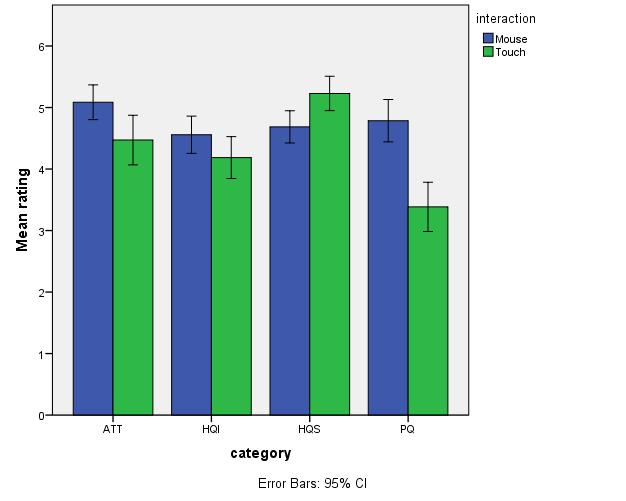
\includegraphics[width=0.5\textwidth]{images/cat_int}
    \label{fig:cat_int}
  }
  \subfigure[]{
    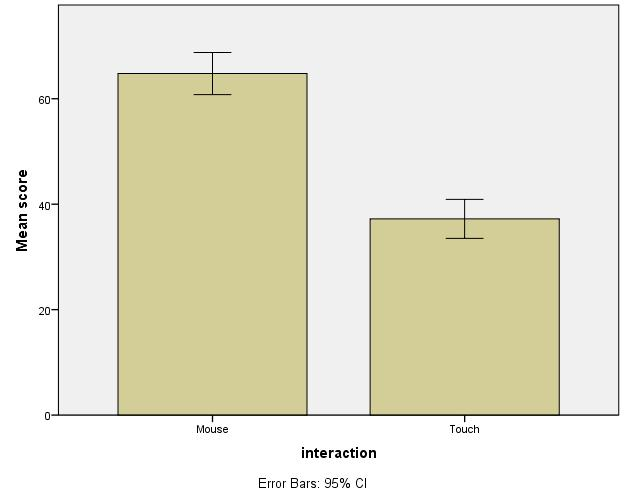
\includegraphics[width=0.5\textwidth]{images/scores}
   \label{fig:scores}
  }
  \caption{(a) The average rating per word pair category, per modality and (b) the average score per modality.}
\end{figure}

%%%%%%%%%%%%%%%%%%%%%%%%%%%%%%%%%%%%%%%%%%%%%%%%%%%%%%%%%%%%%%%%%%%%%%%%%%%%%%%
% Discussion
%%%%%%%%%%%%%%%%%%%%%%%%%%%%%%%%%%%%%%%%%%%%%%%%%%%%%%%%%%%%%%%%%%%%%%%%%%%%%%%
\chapter{Discussion}
\label{chap:discussion}

\section{Research Question}
We have compared the usability of a self-made puzzle game when played on a personal computer and when played on a multi-touch table. For this end, we have performed two usability studies, one for the game on a personal computer and one for on the multi-touch table, and compared the results. Our research question was:\\Will users prefer to use the touch modality or the mouse? \\ \\To which our hypothesis was: \\ \\The user experience with the mult-touch table will be more positive than with the personal computer, unless the accuracy of the multi-touch table is low. \\\\ The results (see section \ref{chap:results}) are mixed. On average, the mouse modality is rated higher on all categories except hedonic stimulation quality. Moreover, the average game score for the touch modality was significantly lower than for the mouse modality. We think both these results can largely be attributed to the inaccuracy of the multi-touch table. It makes sense the performance on the multi-touch table is lower than on the personal computer if the touchtable does not work accurately. During the experiment, we saw people struggling with selecting and dragging objects. This also explains why the touchtable has a lower score of pragmatic quality. We think the fact that the touchtable scores lower on Attractiviness can be explained by the low resolution of the projected image on the touchtable. The projection was not as clear as the screen of the personal computer we ran the mouse modality on. The lower score for the hedonic identity quality on the multi-touch table compared to the personal computer is harder to explain. A possible explanation for this is that the low accuracy of the multi-touch table results in a reduces feeling of control, which results in a reduced ability to identify with the user interface. \\ The one quality on which the touchtable scored higher than the personal computer is Hedonic Stimulation. A possible explanation for this is that the touch modality is more intuitive than the mouse modality. \\ 

\section{Future Research}
There are several possibilities for extending research to our experiment.
Firstly, it would be interesting to repeat the experiment with test subjects without any experience with a mouse.
This would provide a better comparison of how intuitive the touch modality is compared to the mouse modality, because most users have a lot of experience with the mouse. This could provide a better answer as to which modality is more intuitive initially. Another possible extension to our research is to repeat it with a more professional, better working multi-touch table. This way we could investigate whether users prefer a personal computer or a multi-touch table without the low accuracy of the touchtable spoiling the experiment. 

%%%%%%%%%%%%%%%%%%%%%%%%%%%%%%%%%%%%%%%%%%%%%%%%%%%%%%%%%%%%%%%%%%%%%%%%%%%%%%%
% Appendix
%%%%%%%%%%%%%%%%%%%%%%%%%%%%%%%%%%%%%%%%%%%%%%%%%%%%%%%%%%%%%%%%%%%%%%%%%%%%%%%
\appendix
\chapter{Collaboration}
\label{chap:collaboration}

In this appendix we will give a quantitative estimate of the amount of work done by each member of the group.
Note that our initial intention for the project was to communicate with the multi-touch table using smartphones.
For this purpose, we had to develop an Android application for the smartphones and set up a server for the Android application to communicate with the multi-touch table.
Despite the fact that we did not manage to make this work in time, a lot of work has been spent on this.

\noindent
 \begin{tabular}{ l c c c r }                               
  \textbf{Time spent working on:}  & Bas Bootsma & Bas Kooiker & Roland Meertens & Thomas Planting \\
  Game& 60 & 0 &  65&30\\
  Multi-touch table& 0 & 0&11&0 \\
  Android application& 0 & 40&0&0 \\
  Server &16 & 0 &0&0\\
  Usability study&0&8&0&0\\
  Report &8 & 10&8&20\\
  Meetings/mail &6&6&6&6\\
  Total&90&64&90&56\\
\end{tabular}

%%%%%%%%%%%%%%%%%%%%%%%%%%%%%%%%%%%%%%%%%%%%%%%%%%%%%%%%%%%%%%%%%%%%%%%%%%%%%%%
% Bibliography
%%%%%%%%%%%%%%%%%%%%%%%%%%%%%%%%%%%%%%%%%%%%%%%%%%%%%%%%%%%%%%%%%%%%%%%%%%%%%%%
\bibliographystyle{plain}
\bibliography{aHCIReport}
\end{document}
